\documentclass[a4paper,11pt,spanish, twoside, leqno]{tfg-uam}

\usepackage[utf8]{inputenc}
\usepackage{amsfonts, amssymb, amsmath, amsthm}
\usepackage{graphicx}
\usepackage{color}

\newtheorem{teor}{Teorema}[chapter]
\newtheorem{lema}[teor]{Lema}
\newtheorem*{teorsin}{Teorema}


\theoremstyle{definition}
\newtheorem{defin}[teor]{Definici\'on}

\title{Teorema de clasificación de superficies}
\author{Rodrigo De Pool}
\tutor{Javier Aramayona}
\curso{2019-2020}


%%%%%METADATOS: rellenar la info solicitada entre llaves
\usepackage{hyperref}
\hypersetup{
	pdfinfo={
            Title={Teorema de clasificaci\'on de superficies }, %Titulo del trabajo; ejemplo: Matematicas y desarrollo
            Author={ Rodrigo De Pool}, %Autor del trabajo; ejemplo: Juan Sanchez
            Director1={javier.aramayona }, %Tutor1: en formato nombre.apellido, tal como aparece en la primera parte, antes de la arroba,  de su direcci�n de correo electr�nico de la UAM; ejemplo: fernando.soria
            Director2={ }, %Tutor2: en formato nombre.apellido, tal como aparece en la primera parte, antes de la arroba,  de su direcci�n de correo electr�nico de la UAM
            Ndirectores={1 }, %Numero total de directores: 1 � 2
            Tipo={TFG}, %no tocar
            Curso={2018-19}, %no tocar
            Palabrasclave={ },% Palabras clave del trabajo, separadas por comas y sin acentos ni espacios; ejemplo: morfismos, formas modulares, ecuaciones elipticas
				}
}
%%%%%%%%%%%%%%%%%%%%%%%%%%%%%%%

\begin{document}




\begin{abstract}[spanish]
Aquí va algo
\end{abstract}
\begin{abstract}[english]
Here goes something
\end{abstract}


\mainmatter
\chapter{Cachos sueltos}



Enunciemos cosas que nos vendrán bien.

Notación de estos cachos sueltos: Utilizaremos una elegante upsilon ($\Upsilon$) para denotar aquello que no sabemos si deberíamos probar formalmente; y usaremos una zeta para aquellas cosas de las que convendría repasar la demostración formal ($\zeta$).

\section{Preliminares de topología}


\begin{defin}\label{defin:noconexo}
	Un conjunto $\mathcal{X}$ es no conexo si existen dos  conjuntos cerrados, $\mathcal{X}_1$ y $\mathcal{X}_2$, tal que $\mathcal{X}=\mathcal{X}_1\cup\mathcal{X}_2$ y $\mathcal{X}_1\cap\mathcal{X}_2=\emptyset$.
\end{defin}


\begin{defin}\label{defin:conexo}
	Un conjunto $\mathcal{X}$ se dice conexo si no cumple la definición anterior.
\end{defin}



\begin{defin}\label{defin:topologiaCociente}
	Sea $\mathcal{X}$ un espacio topológico con topología $\mathcal{T}_X$, sea $\mathcal{Y}$ un conjunto, y $f$ una función  $f:\mathcal{X}\longrightarrow\mathcal{Y}$. Entonces definimos la topología cociente:
	\begin{align*}
	\mathcal{T}_Y = \{U\subset\mathcal{Y}: f^{-1}(U)\in\mathcal{T}_X\}
	\end{align*} 
	\begin{itemize}
		\item 
		Se puede comprobar $T_Y$ genera en efecto una topología de $Y$
		\item
		$T_Y$ es la topología más fina que hace continua a $f$
		\item 
		Es usual trabajar con $Y$ como una partición o conjunto de clases de equivalencia de $X$
	\end{itemize}
\end{defin}


\begin{lema}\label{lema:conexoAconexo}
	Sean $X$ e $Y$ espacios topológicos y $f: X \longrightarrow Y$ continua, entonces: 
	\begin{align*}
	X \textrm{ conexo} \Rightarrow Y \textrm{conexo}
	\end{align*}
\end{lema}


\begin{lema}\label{lema:compactoAcompacto}
	Sean $X$ e $Y$ espacios topológicos y $f: X \longrightarrow Y$ continua, entonces: 
	\begin{align*}
	X \textrm{ compacto} \Rightarrow f(X) \textrm{ compacto}
	\end{align*}
	Claramente, si $f$ cumple también ser sobreyectiva entonces $Y$ será compacto.
\end{lema} 



\begin{lema}\label{lema:XcompactoYt2fcontinua}
	Sean $X$ e  $Y$ espacios topológicos, $X$ un compacto, $Y$ un espacio de Haussdorf y $f: X \longrightarrow Y$ continua y sobreyectiva , entonces $f$ es cerrada.
	
	Corolario: Se cumple, además, que la topología de $Y$ es la topología cociente.
\end{lema}


\section{Definiciones}


\begin{defin}\label{defin:nvariedad}
	Una n-variedad es un espacio topológico de Haussdorff tal que todo punto tiene un entorno abierto homeomorfo a la bola abierta n-dimensional.
\end{defin}



\begin{defin}\label{defin:superficie}
	A una 2-variedad conexa la llamaremos superficie.
\end{defin}

Introducimos a continuación algunos ejemplos característicos de superficies:
\begin{defin}\label{defin:toro}
	Se llama toro al cuadrado unidad:
	\begin{align*}
		X = \left\{(x,y): 0\leq x\leq 1, 0\leq y\leq 1  \right\} 
	\end{align*}
	Identificando los puntos:
	\begin{itemize}
		\item 
		$(x,1)$ con $(x,0)$ para $0\leq x\leq 1$
		\item 
		$(0,y)$ con $(1,y)$ para $0\leq y\leq 1$
	\end{itemize}
La topología que se considera es la cociente, inducida por el cuadrado cerrado con la topología usual.
\end{defin}



Para considerar gráficamente el toro se asigna a cada arista de un cuadrado unidad una letra y un sentido. Si dos aristas comparten letra, entonces son puntos identificados según el sentido de la flecha. Mostramos en \ref{fig:toro} la representación visual del toro.

\begin{figure}[h]\label{fig:toro}
	\centering
	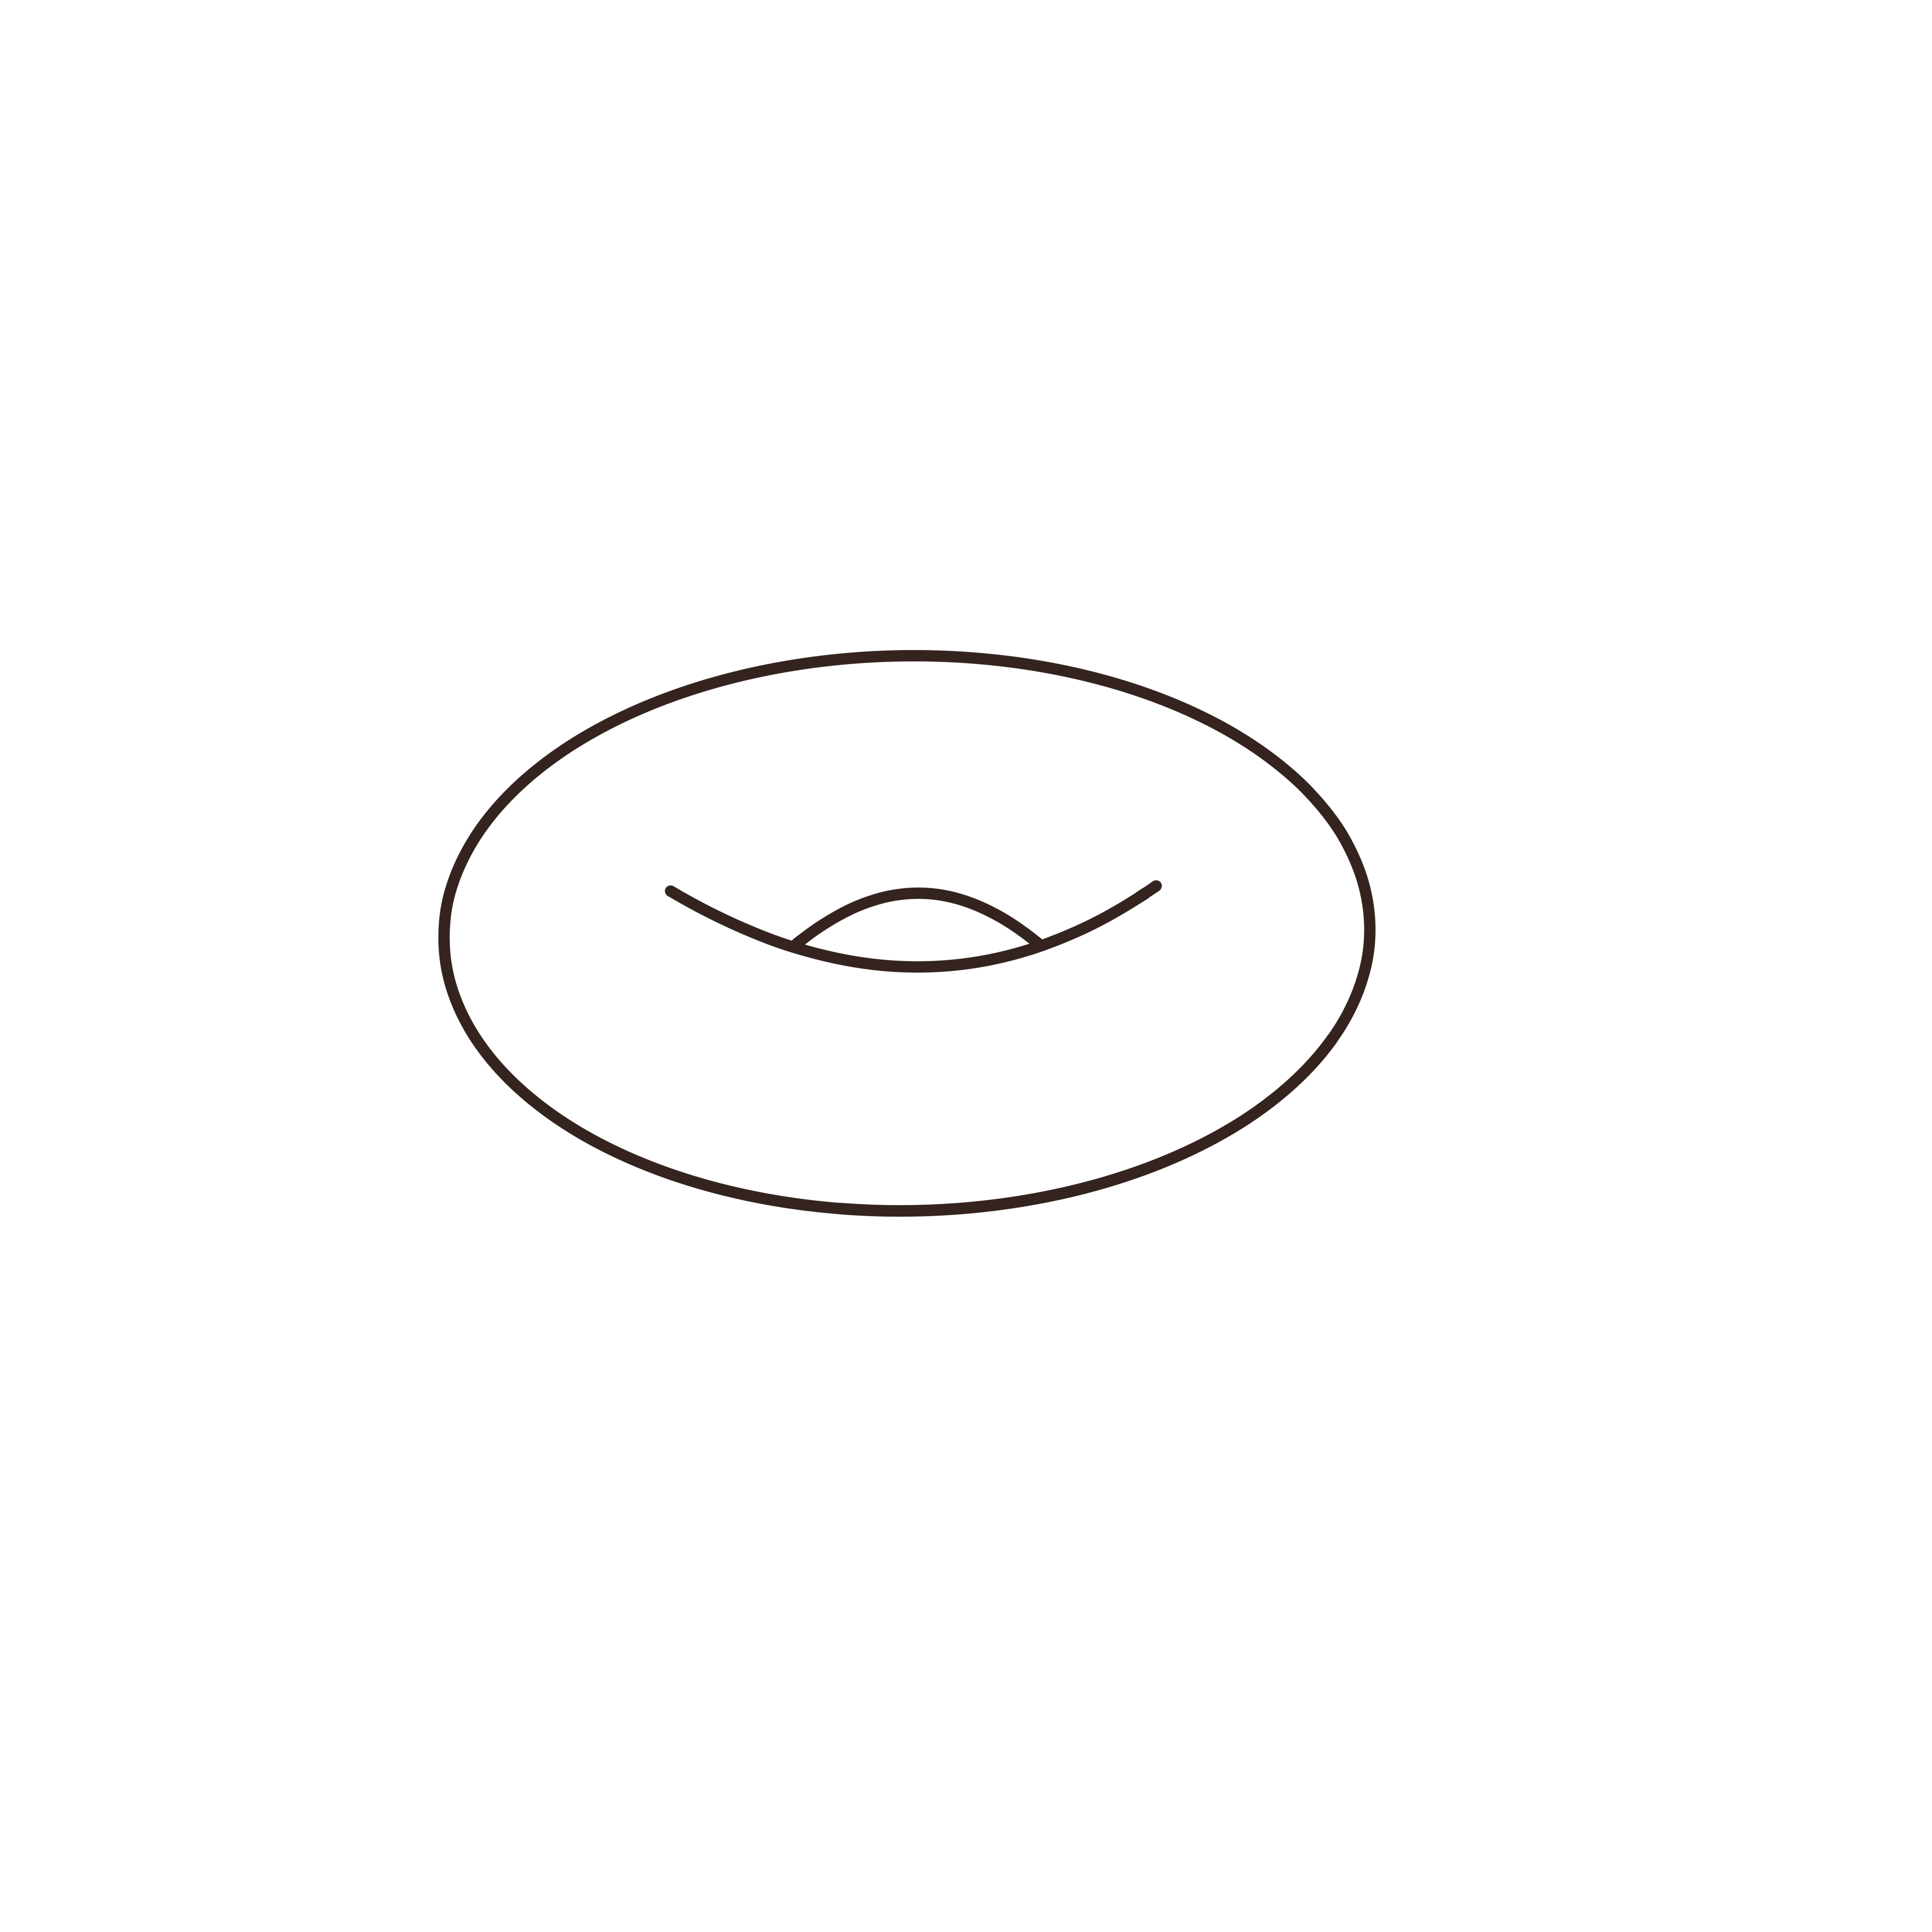
\includegraphics[width=0.3\linewidth]{imagenes/toro.png}
	\caption{Toro}
\end{figure} 

Partiendo de la notación gráfica se puede establecer una notación algebraica. Empezando en uno de los vértices recorremos el borde de la figura en el sentido de las agujas del reloj, si el sentido  de la arista corresponde con el del recorrido entonces escribimos la letra, si es contrario entonces escribimos la letra elevado a -1. En el caso del toro tenemos: $aba^{-1}b^{-1}$ 



\begin{defin}\label{defin:planoproyectivo}
	Se llama plano proyectivo al cuadrado unidad, identificando los puntos:
	\begin{itemize}
		\item 
		$(x,1)$ con $(1-x,0)$ para $0\leq x\leq 1$
		\item 
		$(0,y)$ con $(1,1-y)$ para $0\leq y\leq 1$
	\end{itemize}
	La topología que se considera es la cociente, inducida por el cuadrado cerrado con la topología usual.
\end{defin}

En la figura \ref{fig:planoproyectivo} observamos el plano proyectivo en notación visual.

\begin{figure}[h]\label{fig:planoproyectivo}
	\centering
	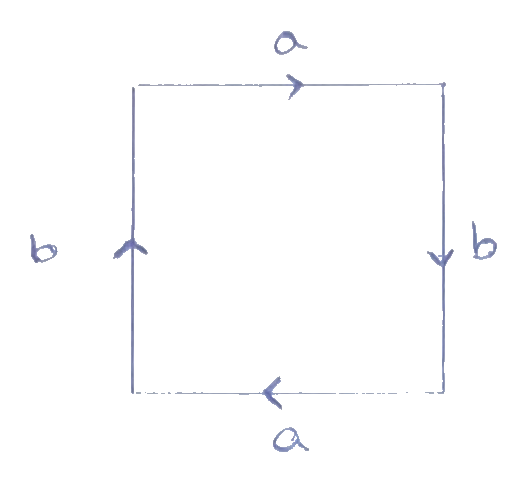
\includegraphics[width=0.3\linewidth]{imagenes/planop.png}
	\caption{Plano proyectivo}
\end{figure} 
En notación algebraica el plano proyectivo se escribe $abab$.

Sirviéndonos de la notación algebraica podemos definir \textit{la botella de Klein} como $aba^{-1}b$ 


\begin{figure}[h]\label{fig:botelladeklein}
	\centering
	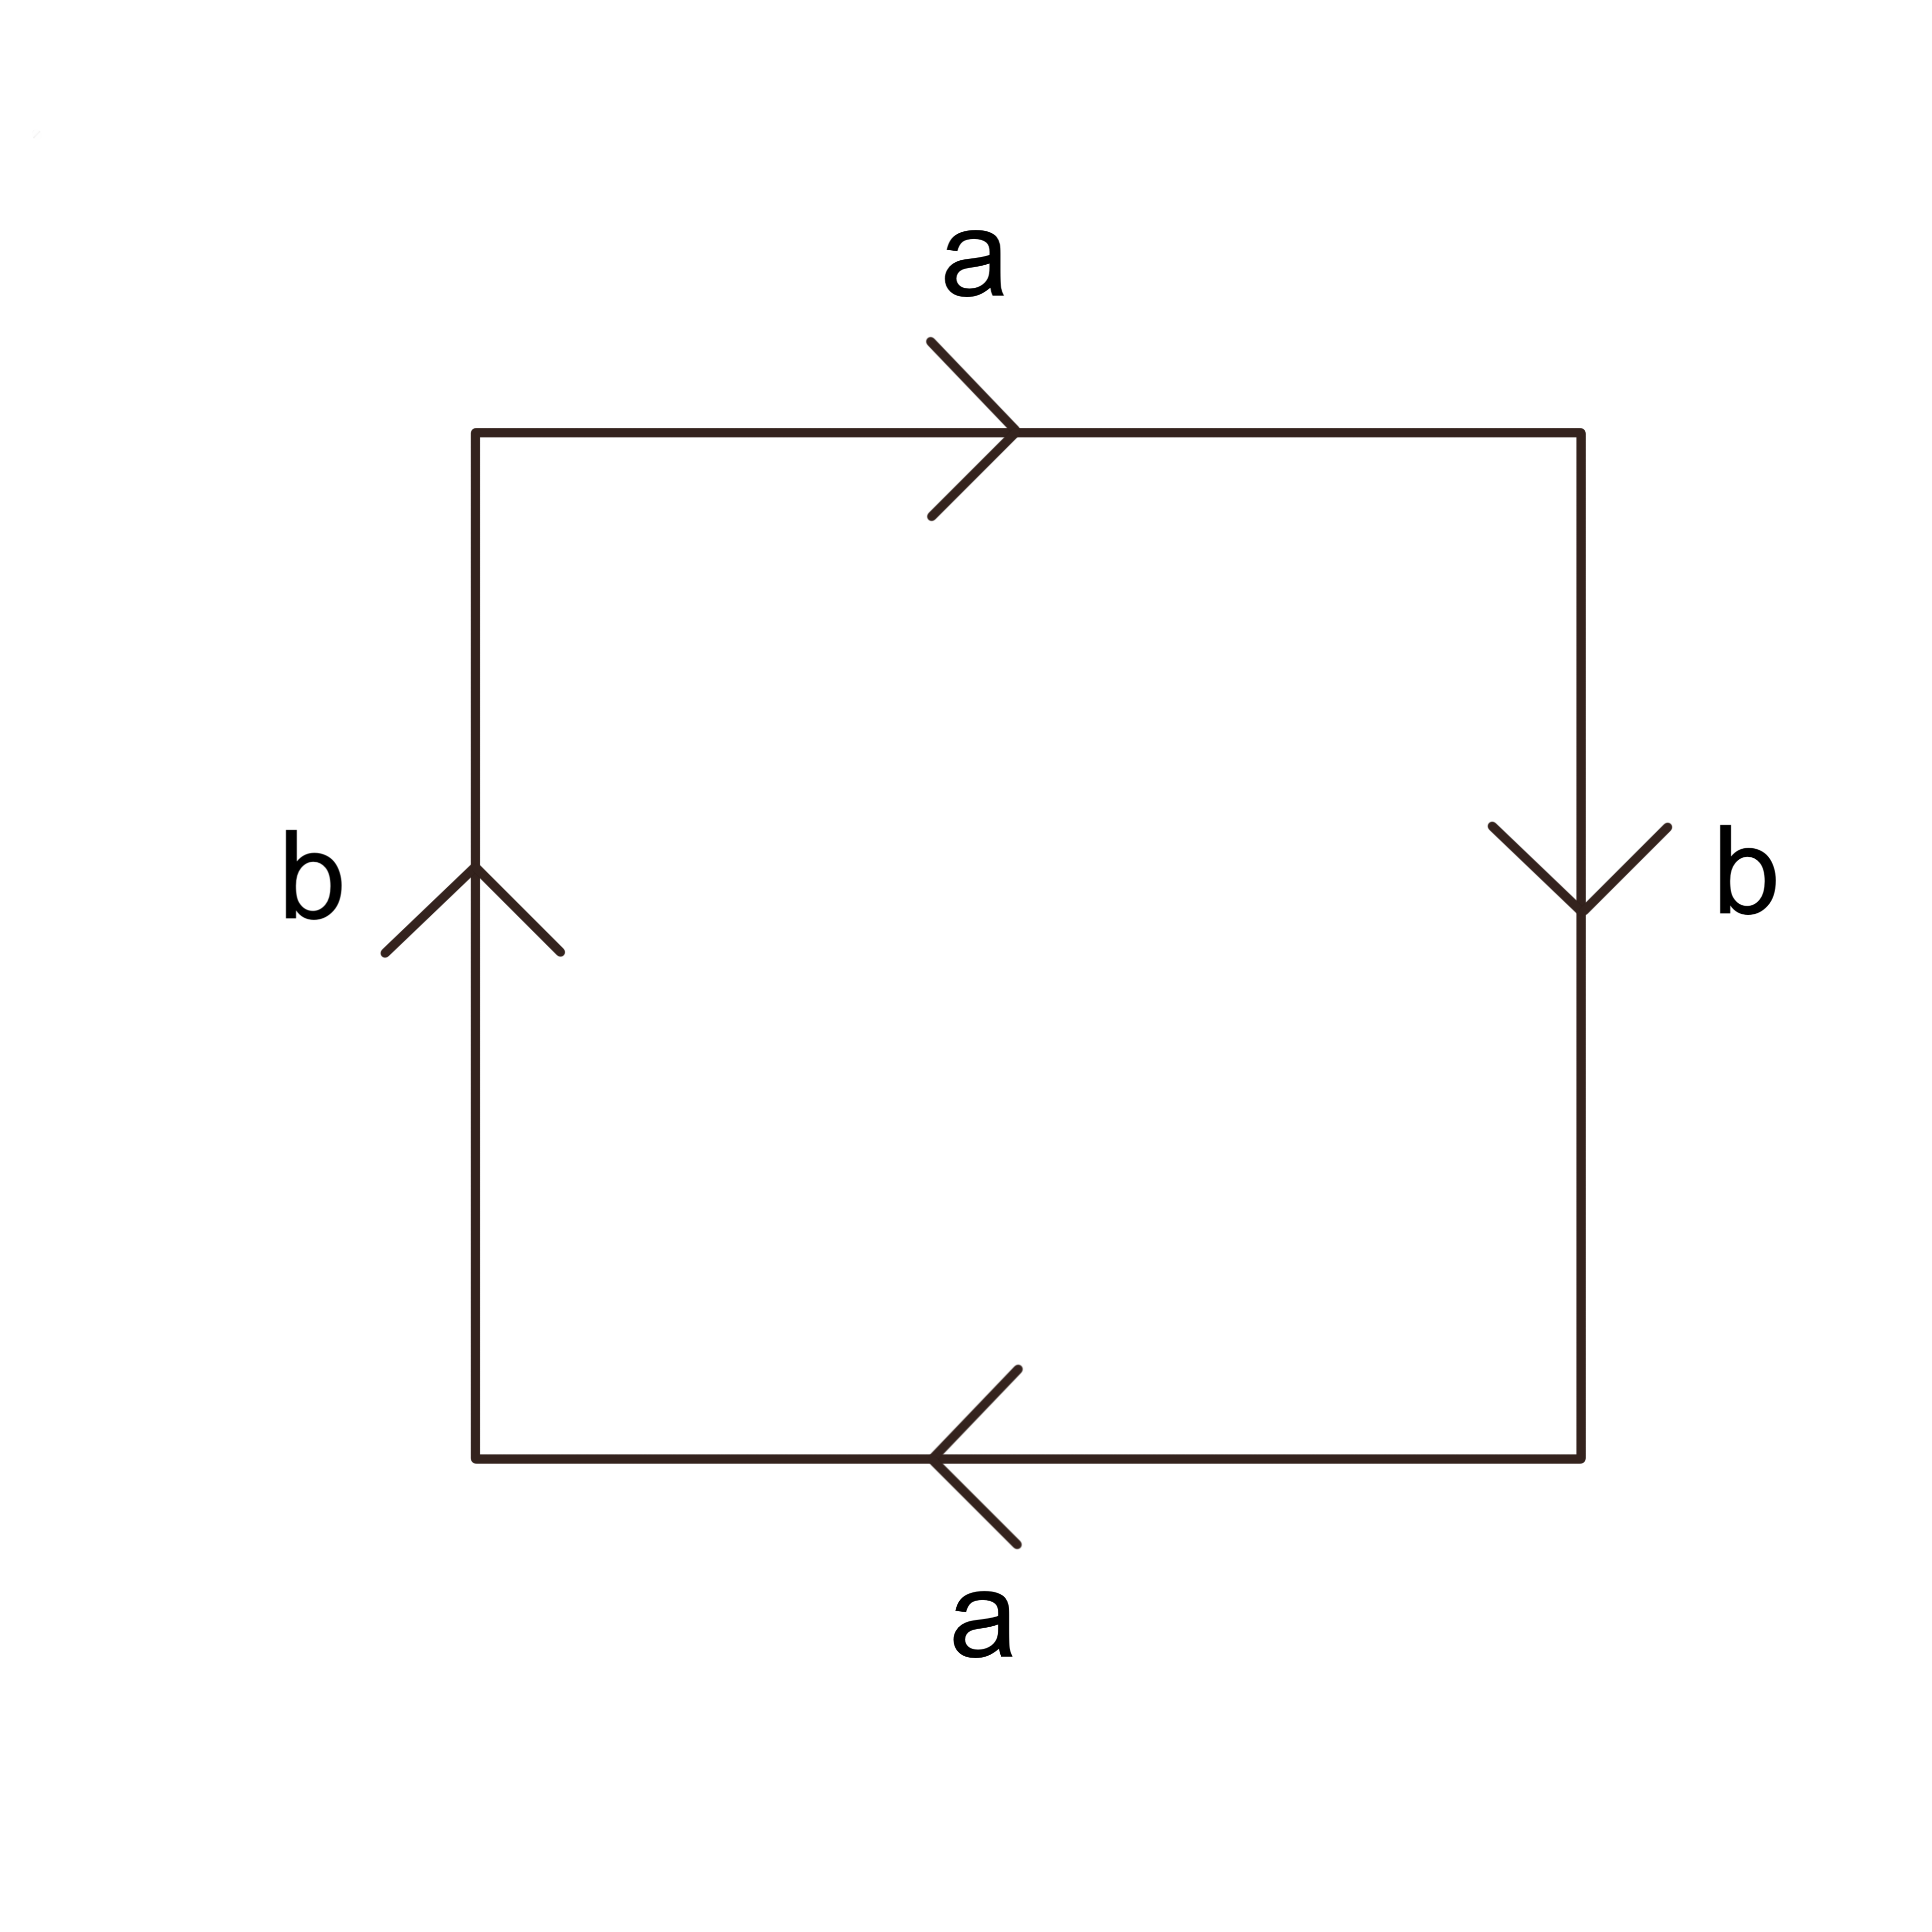
\includegraphics[width=0.3\linewidth]{imagenes/klein.png}
	\caption{Botella de Klein}
\end{figure} 


\begin{defin}\label{defin:sumaconexa}
	Dadas dos superfices $S_1$ y $S_2$ podemos definir la suma conexa de ambas, $S_1\#S_2$, como la superficie generada a partir de los siguientes pasos:
	
	\begin{enumerate}
		\item 
		Para cada $S_i$ tomamos un subconjunto $D_i\subset S_i$ homeomorfo al disco cerrado de dos dimensiones $E^2$. Llamamos $S'_i$ al complementario del interior de $D_i$.
		\item 
		Sea $\phi_i$ el homeomorfismo que manda $D_i$ al disco cerrado $E^2$, definimos el homeomorfismo $\psi$ que manda la frontera de $D'_1$ a la frontera de $D'_2$ como:
		\begin{align*}
		\psi = ((\phi_{2}\mid_{fr(D_2)})^{-1}) \circ (\phi_1\mid_{fr(D_1)})
		\end{align*}
		\item 
		Definimos entonces $S_1\#S_2$ como $S'_1\cup S'_2$ dotado de la topología cociente que resulta de identificar los puntos $x$ y $\psi(x)$ para todo punto de la frontera de $D_1$.
	\end{enumerate}
	
	Para confirmar la validez de estar definición hay que aclarar varios puntos:
	\begin{enumerate}
		\item 
		Primero, por qué podemos asegurar en el punto 1 de la definición que existe un subconjunto homeomorfo a un disco.
		\begin{proof}
			Tomamos un punto $p\in S_i$ cualquiera. Como $S_i$ es una 2-variedad, entonces existe un homeomorfismos $g$ que manda un entorno, $U$, del punto $p$ al círculo abierto. 
			
			Tomamos $E_{\frac{1}{2}}$ el disco cerrado de radio $\frac{1}{2}$, y $U'= g^{-1}(E_{\frac{1}{2}})$. Tenemos que $g\mid_{U'}$ es un homeomorfismo de un subconjunto de $S_i$ a $E_{\frac{1}{2}}$ que a su vez es homeomorfo al disco cerrado de radio 1. (HACE FALTA?)
		\end{proof} 
		\item 
		Segundo, tenemos que asegurarnos que en el punto 2 las fronteras de $D_1$ y $D_2$ tienen la misma imagen.
		\begin{proof}
			Comencemos por aclarar una sutileza en la definición: Cuando hablamos de $D_i$ homeomorfos a $E^2$, nos referimos a homeomorfos como subconjuntos de las superficies, no como conjuntos independientes dotados de la topología del subconjunto.
			
			Partiendo de eso, basta con probar que dado un homeomorfismo $f: X\longrightarrow Y$, y el conjunto cerrado $B\subset X$, entonces $f(fr(B)))= fr(f(B))$.
			Para esto basta con probar que dado un homeomorfismo $f: U\subset X \longrightarrow V\subset Y$, con $U$ y $V$ cerrados, se cumple que $f(fr(U)) = fr(V)$. Esto se sigue directamente de que $f(\mathring{B})=\mathring{f(B)}$, que a su vez es resultado inmediato de las propiedades de homeomorfismos. (HACE FALTA?)
		\end{proof}
		\item 
		Tercero, habría que comprobar que, en efecto, el objeto obtenido es una superficie. Es decir, comprobar que todo punto tiene un entorno homeomorfo al disco abierto, que el espacio es T2 y que es conexo.
		\begin{proof}
			
			(HACE FALTA?)
		\end{proof}
		\item 
		Y, finalmente, tenemos que comprobar que esta definición es independiente de los conjuntos $D_i$ escogidos e independiente de los homeomorfismos.
		\begin{proof}
			(HACE FALTA?)
		\end{proof}
	\end{enumerate} 
\end{defin}

\begin{lema}{El pseudolema más útil de toda la topología}
	
	Al dilatar, comprimir, trasladar y cortar-identificar una figura, el objeto obtenido es homeomorfo al inicial. ¿Por qué?, se pregunta un matemático, porque todas las transformaciones son continuas. (¿Incluir en el TFG en tono seriesisímo?) 
\end{lema}

¿Ejemplillos de suma conexa de toros y planos proyectivos?

\begin{lema}\label{lema:sumadedosplanosproyectivos}
	La suma conexa de dos planos proyectivos es una botella de Klein.
	\begin{proof}
		Un plano proyectivo se puede entender como el disco unidad en el que se identifican los puntos diametralmente opuestos. Utilizando esta definición seleccionamos el subconjunto $D = \left\{(x,y): |y|\geq\frac{1}{2}, |x|\leq\sqrt{1-y^2} \right\}$, homeomorfo al disco cerrado, para realizar la suma conexa de los planos. En la figura  \ref{fig:parte1SumaConexaDePlanosP} eliminamos el conjunto $D$ e indicamos con líneas discontinuas los segmentos a identificar con la otra superficie.
		
		\begin{figure}[h]\label{fig:parte1SumaConexaDePlanosP}
			\centering
			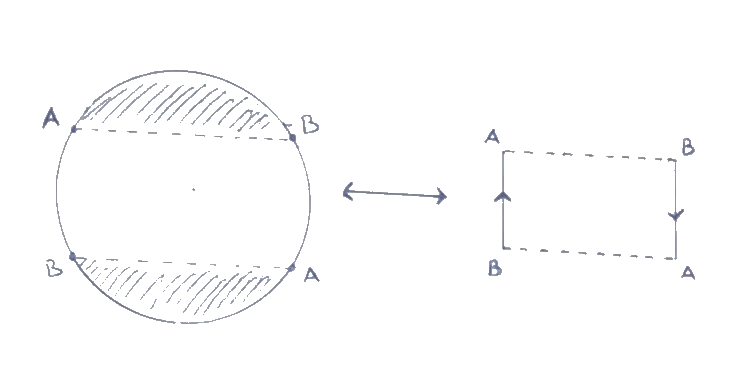
\includegraphics[width=0.7\linewidth]{imagenes/p1planop.png}
			\caption{Plano proyectivo menos un subconjunto homemorfo al disco cerrado}
		\end{figure} 
	
		Tomamos entonces dos planos proyectivos $I$ e $II$ y realizamos la suma conexa:
		
		\begin{figure}[h]\label{fig:sumaconexadepps}
			\centering
			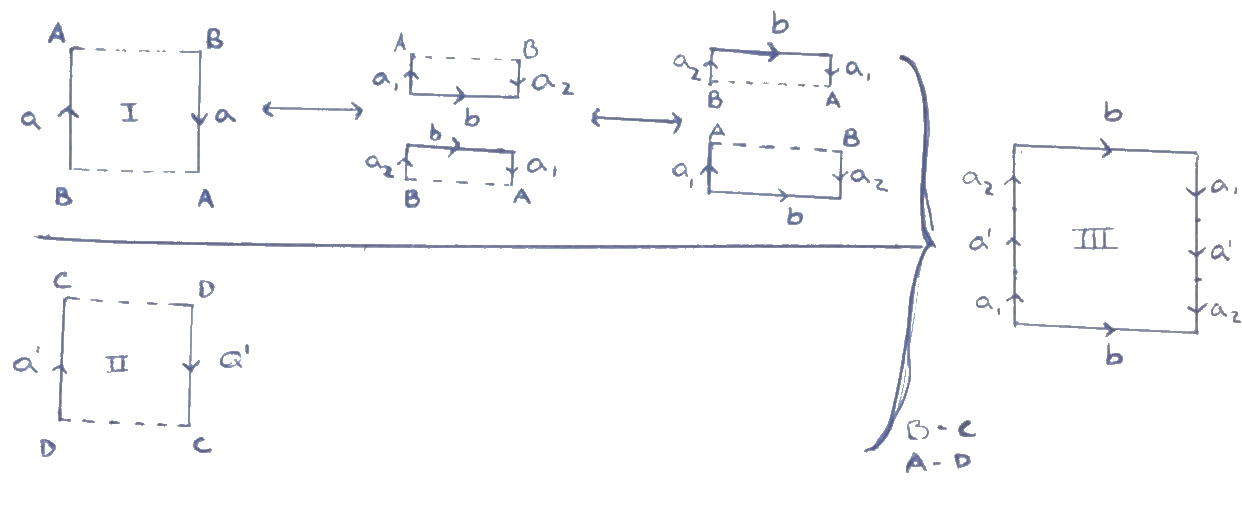
\includegraphics[width=0.8\linewidth]{imagenes/sumapps.png}
			\caption{Suma conexa de planos proyectivos}
		\end{figure} 
		La figura final obtenida ($III$) es una \textit{Botella de Klein}.
	\end{proof}
\end{lema}







\begin{defin}\label{defin:triangulacion}
	Una triangulación de una superficie compacta, $S$, consiste en subconjuntos cerrados, ${T_1, ..., T_n}$, que cubren a $S$ y una familia de homeomorfismos, ${\phi_1, ..., \phi_n}$, que cumplen:
	\begin{align*}
	\phi_i: T'_i \longrightarrow T_i
	\end{align*}
	Donde $T'_i$ es un triángulo del plano $\mathbb{R}^2$. Además, tomando $T_i$ y $T_j$ con $i\neq j$, se cumple una de las siguientes condiciones:
	\begin{itemize}
		\item 
		Son conjuntos totalmente disjuntos.
		\item 
		Comparten un solo vértice en común y solo eso (Llamamos vértice a todo elemento de $S$ que se corresponde por algún $\phi_i$ con un vértice en el plano).
		\item 
		Tienen toda una arista en común y solo eso (Llamamos arista a la imagen de una arista de alguún $T'_i$ por $\phi_i$).
	\end{itemize}
\end{defin}


\begin{teor}{Teorema de Tibor Radó}\label{teor:teoremaDeTriangulacion}
	
	Toda $S$ superficie compacta es triangulable.
\end{teor}(NO LO DEMOSTRAREMOS)




Lemas de triangulación
\begin{lema}\label{lema:lema1detriangulacion}
	Sea $S$ una superficie triangulable entonces una arista lo es de exactamente dos triángulos.
\end{lema}(TODO: FALTA DEMS)

\begin{lema}\label{lema:lema2detriangulacion}
	Sea  $S$ una superficie triangulable y $v\in S$ un vértice en esa triangulación, entonces podemos ordenar el conjunto de todos los triángulos con vértice $v$ cíclicamente,  $T_0, T_1, ..., T_n = T_0$, de manera que $T_i$ y $T_{i+1}$ tienen toda una arista en común para todo $0\leq i\leq n-1$.
\end{lema}(TODO: FALTA DEMS)





(EJEMPLO DE SUMA DE CONEXA DE PLANO PROY CON PLANO PROY DA BOTELLA DE KLEIN)
(TEOREMA FINALLLL)

\begin{teor}{Teorema de clasificación de superficies compactas}\label{teor:teoremadeclasificacion}
	
	Toda superficie compacta es homeomorfa a una esfera, a una suma conexa de toros o una suma conexa de planos proyectivos.
\end{teor}









\chapter{Introducci\'on y preliminares}\label{chap1}
\setcounter{page}{1}

Dada una superficie, concepto que se formalizará posteriormente, es razonable preguntarse por otras superficies que sean topológicamente equivalentes. Intuitivamente, lo que se estaría buscando es una clasificación que nos indique qué otras superficies se pueden conseguir al deformar continuamente una superficie dada. El objetivo de este trabajo es dar una expresión explícita a tal clasificación y, mediante una demostración constructiva, dar un método para conseguir la clase de equivalencia topológica de una superficie cualquiera.

Para recabar todos los elementos necesarios en la demostración, el trabajo sigue la siguiente estructura:
\begin{itemize}\itemsep=0pt
\item
Mencionamos algunos lemas básicos de la asignatura de topología que se utilizarán durante la demostración.

\item
Introducimos las definiciones necesarias para formalizar el teorema objeto de nuestro trabajo.
\item
Enunciamos y demostramos algunos teoremas que serán necesarios posteriormente.
\item
Finalmente, procedemos a enunciar y demostrar el teorema de clasificación de superficies compactas.
\end{itemize}

Bla bla, funcionamiento de las citas: \cite{Abel} y \cite{S-W}.

\section{Introducci\'on}

Pruebas de como funciona todo
\begin{equation}\label{eq1}
e^{i\pi }+1=0.
\end{equation}

mas cosas
\begin{equation}\label{eq2}
e^{i\pi }+1=0.
\end{equation}
Integer tincidunt. Cras dapibus.
\begin{equation}\label{eq3}
e^{i\pi }+1=0.
\end{equation}
Referencias a ecuaciones \eqref{eq1}--\eqref{eq2}, et \eqref{eq3}. 




\begin{teorsin}
[Cauchy--Schwarz]Nullam quis ante. 
\end{teorsin}


\begin{teor}\label{teor1}
Nullam quis ante. Etiam sit amet orci eget eros faucibus tincidunt. Duis leo. Sed fringilla mauris sit amet nibh. Donec sodales sagittis magna. Sed consequat, leo eget bibendum sodales, augue velit cursus nunc.
\end{teor}



\begin{lema}\label{lema1}
Nullam quis ante. Etiam sit amet orci eget eros faucibus tincidunt. Duis leo. Sed fringilla mauris sit amet nibh. Donec sodales sagittis magna. Sed consequat, leo eget bibendum sodales, augue velit cursus nunc.
\end{lema}

\begin{proof}
Nullam quis ante. 
\end{proof}


\begin{lema}\label{lema2}
Nullam quis ante. Etiam sit amet orci eget eros faucibus tincidunt. Duis leo. Sed fringilla mauris sit amet nibh. Donec sodales sagittis magna. Sed consequat, leo eget bibendum sodales, augue velit cursus nunc.
\end{lema}

Lorem ipsum dolor sit amet, consectetuer adipiscing elit. Aenean commodo ligula eget dolor. Aenean massa. Cum sociis natoque penatibus et magnis dis parturient montes, nascetur ridiculus mus. Donec quam felis, ultricies nec, pellentesque eu, pretium quis, sem. Nulla consequat massa quis enim. Donec pede justo, fringilla vel, aliquet nec, vulputate eget, arcu. In enim justo, rhoncus ut, imperdiet a, venenatis vitae, justo. Nullam dictum felis eu pede mollis pretium. Integer tincidunt. Cras dapibus. Vivamus elementum semper nisi. Aenean vulputate eleifend tellus. Aenean leo ligula, porttitor eu, consequat vitae, eleifend ac, enim. Aliquam lorem ante, dapibus in, viverra quis, feugiat a, tellus. Phasellus viverra nulla ut metus varius laoreet. Quisque rutrum. Aenean imperdiet. Etiam ultricies nisi vel augue. Curabitur ullamcorper ultricies nisi. Nam eget dui. Etiam rhoncus. Maecenas tempus, tellus eget condimentum rhoncus, sem quam semper libero, sit amet adipiscing sem neque sed ipsum. Nam quam nunc, blandit vel, luctus pulvinar, hendrerit id, lorem. Maecenas nec odio et ante tincidunt tempus. Donec vitae sapien ut libero venenatis faucibus. Nullam quis ante. Etiam sit amet orci eget eros faucibus tincidunt. Duis leo. Sed fringilla mauris sit amet nibh. Donec sodales sagittis magna. Sed consequat, leo eget bibendum sodales, augue velit cursus nunc.


\begin{proof}[\sc Demostraci\'on del lema {\rm \ref{lema2}}]
Nullam quis ante:
\begin{equation}
2+2=4.\qedhere
\end{equation}
\end{proof}

\section{Resultados preliminares}

Lorem ipsum dolor sit amet, Teorema \ref{teor1}, consectetuer adipiscing elit. Aenean commodo ligula eget dolor. Aenean massa. Cum sociis natoque penatibus et magnis dis parturient montes, nascetur ridiculus mus. Donec quam felis, ultricies nec, pellentesque eu, pretium quis, sem. Nulla consequat massa quis enim. Donec pede justo, fringilla vel, aliquet nec, vulputate eget, arcu. In enim justo, rhoncus ut, imperdiet a, venenatis vitae, justo. Nullam dictum felis eu pede mollis pretium. Integer tincidunt. Cras dapibus. Vivamus elementum semper nisi. Aenean vulputate eleifend tellus. Aenean leo ligula, porttitor eu, consequat vitae, eleifend ac, enim. Aliquam lorem ante, dapibus in, viverra quis, feugiat a, tellus. Phasellus viverra nulla ut metus varius laoreet. Quisque rutrum. Aenean imperdiet. Etiam ultricies nisi vel augue. Curabitur ullamcorper ultricies nisi. Nam eget dui. Etiam rhoncus. Maecenas tempus, tellus eget condimentum rhoncus, sem quam semper libero, sit amet adipiscing sem neque sed ipsum. Nam quam nunc, blandit vel, luctus pulvinar, hendrerit id, lorem. Maecenas nec odio et ante tincidunt tempus. Donec vitae sapien ut libero venenatis faucibus. Nullam quis ante. Etiam sit amet orci eget eros faucibus tincidunt. Duis leo. Sed fringilla mauris sit amet nibh. Donec sodales sagittis magna. Sed consequat, leo eget bibendum sodales, augue velit cursus nunc,
\begin{align}\label{eq4}
&e^{i\pi }+1=0,
\\
&2e^{i\pi }+2=0.\label{eq5}
\end{align}

Lorem ipsum dolor sit amet, consectetuer adipiscing elit. Aenean commodo ligula eget dolor.
\begin{align}\nonumber
0&=e^{i\pi }+1=e^{i\pi }+1=e^{i\pi }+1=e^{i\pi }+\sum_{n=1}^\infty \frac{1}{2^n}
\\
&=-1+\sum_{n=1}^\infty \frac{1}{2^n}=-1+1=0.\label{eq6}
\end{align}
et
\begin{equation}\label{eq7}
\begin{aligned}
e^{i\pi }+1=0,
\\
e^{i\pi }+1=0.
\end{aligned}
\end{equation}


Lorem ipsum dolor sit amet, consectetuer adipiscing elit. Aenean commodo ligula eget dolor.
\begin{align*}
e^{i\pi }+1&=0,
\\
e^{i\pi }+1&=0.
\end{align*}
Aenean massa: 
\begin{equation}
\left\{
\begin{array}{l}
e^{i\pi }+1=0,
\\
e^{i\pi }+1=0.
\end{array}
\right.
\end{equation}


Cum sociis natoque penatibus et magnis dis parturient montes, nascetur ridiculus mus. Donec quam felis, ultricies nec, pellentesque eu, pretium quis, sem. Nulla consequat massa quis enim. Donec pede justo, fringilla vel, aliquet nec, vulputate eget, arcu. In enim justo, rhoncus ut, imperdiet a, venenatis vitae, justo. Nullam dictum felis eu pede mollis pretium. Integer tincidunt. Cras dapibus. Vivamus elementum semper nisi. Aenean vulputate eleifend tellus. Aenean leo ligula, porttitor eu, consequat vitae, eleifend ac, enim. Aliquam lorem ante, dapibus in, viverra quis, feugiat a, tellus. Phasellus viverra nulla ut metus varius laoreet. Quisque rutrum. Aenean imperdiet. Etiam ultricies nisi vel augue. Curabitur ullamcorper ultricies nisi. Nam eget dui. Etiam rhoncus. Maecenas tempus, tellus eget condimentum rhoncus, sem quam semper libero, sit amet adipiscing sem neque sed ipsum. Nam quam nunc, blandit vel, luctus pulvinar, hendrerit id, lorem. Maecenas nec odio et ante tincidunt tempus. Donec vitae sapien ut libero venenatis faucibus. Nullam quis ante. Etiam sit amet orci eget eros faucibus tincidunt. Duis leo. Sed fringilla mauris sit amet nibh. Donec sodales sagittis magna. Sed consequat, leo eget bibendum sodales, augue velit cursus nunc,

Lorem ipsum dolor sit amet, consectetuer adipiscing elit. Aenean commodo ligula eget dolor. Aenean massa. Cum sociis natoque penatibus et magnis dis parturient montes, nascetur ridiculus mus. Donec quam felis, ultricies nec, pellentesque eu, pretium quis, sem. Nulla consequat massa quis enim. Donec pede justo, fringilla vel, aliquet nec, vulputate eget, arcu. In enim justo, rhoncus ut, imperdiet a, venenatis vitae, justo. Nullam dictum felis eu pede mollis pretium. Integer tincidunt. Cras dapibus. Vivamus elementum semper nisi. Aenean vulputate eleifend tellus. Aenean leo ligula, porttitor eu, consequat vitae, eleifend ac, enim. Aliquam lorem ante, dapibus in, viverra quis, feugiat a, tellus. Phasellus viverra nulla ut metus varius laoreet. Quisque rutrum. Aenean imperdiet. Etiam ultricies nisi vel augue. Curabitur ullamcorper ultricies nisi. Nam eget dui. Etiam rhoncus. Maecenas tempus, tellus eget condimentum rhoncus, sem quam semper libero, sit amet adipiscing sem neque sed ipsum. Nam quam nunc, blandit vel, luctus pulvinar, hendrerit id, lorem. Maecenas nec odio et ante tincidunt tempus. Donec vitae sapien ut libero venenatis faucibus. Nullam quis ante. Etiam sit amet orci eget eros faucibus tincidunt. Duis leo. Sed fringilla mauris sit amet nibh. Donec sodales sagittis magna. Sed consequat, leo eget bibendum sodales, augue velit cursus nunc,


\chapter{El segundo cap\'{\i}tulo}\label{chap2}

Lorem ipsum dolor sit amet, consectetuer adipiscing elit. Aenean commodo ligula eget dolor. Aenean massa. Cum sociis natoque penatibus et magnis dis parturient montes, nascetur ridiculus mus. Donec quam felis, ultricies nec, pellentesque eu, pretium quis, sem. Nulla consequat massa quis enim. Donec pede justo, fringilla vel, aliquet nec, vulputate eget, arcu. In enim justo, rhoncus ut, imperdiet a, venenatis vitae, justo. Nullam dictum felis eu pede mollis pretium. Integer tincidunt. Cras dapibus. Vivamus elementum semper nisi. Aenean vulputate eleifend tellus. Aenean leo ligula, porttitor eu, consequat vitae, eleifend ac, enim. Aliquam lorem ante, dapibus in, viverra quis, feugiat a, tellus.
\begin{equation}\label{eq8}
e^{i\pi }+1=0.
\end{equation}
Phasellus viverra nulla ut metus varius laoreet \eqref{eq1}. Quisque rutrum. Aenean imperdiet. Etiam ultricies nisi vel augue. Curabitur ullamcorper ultricies nisi. Nam eget dui. Etiam rhoncus. Maecenas tempus, tellus eget condimentum rhoncus, sem quam semper libero, sit amet adipiscing sem neque sed ipsum. Nam quam nunc, blandit vel, luctus pulvinar, hendrerit id, lorem. Maecenas nec odio et ante tincidunt tempus. Donec vitae sapien ut libero venenatis faucibus. Nullam quis ante. Etiam sit amet orci eget eros faucibus tincidunt. Duis leo. Sed fringilla mauris sit amet nibh. Donec sodales sagittis magna. Sed consequat, leo eget bibendum sodales, augue velit cursus nunc,
$$
e^{i\pi }+1=0.
$$

Lorem ipsum dolor sit amet, consectetuer adipiscing elit. Aenean commodo ligula eget dolor. Aenean massa. Cum sociis natoque penatibus et magnis dis parturient montes, nascetur ridiculus mus. Donec quam felis, ultricies nec, pellentesque eu, pretium quis, sem. Nulla consequat massa quis enim. Donec pede justo, fringilla vel, aliquet nec, vulputate eget, arcu. In enim justo, rhoncus ut, imperdiet a, venenatis vitae, justo. Nullam dictum felis eu pede mollis pretium.
\begin{equation}
e^{i\pi }+1=0.
\end{equation}
Integer tincidunt. Cras dapibus. Vivamus elementum semper nisi. Aenean vulputate eleifend tellus. Aenean leo ligula, porttitor eu, consequat vitae, eleifend ac, enim. Aliquam lorem ante, dapibus in, viverra quis, feugiat a, tellus. Phasellus viverra nulla ut metus varius laoreet. Quisque rutrum. Aenean imperdiet. Etiam ultricies nisi vel augue. Curabitur ullamcorper ultricies nisi.
\begin{equation}
e^{i\pi }+1=0.
\end{equation}
Nam eget dui. Etiam rhoncus. Maecenas tempus, tellus eget condimentum rhoncus, sem quam semper libero, sit amet adipiscing sem neque sed ipsum. Nam quam nunc, blandit vel, luctus pulvinar, hendrerit id, lorem. Maecenas nec odio et ante tincidunt tempus. Donec vitae sapien ut libero venenatis faucibus. Nullam quis ante. Etiam sit amet orci eget eros faucibus tincidunt. Duis leo. Sed fringilla mauris sit amet nibh. Donec sodales sagittis magna. Sed consequat, leo eget bibendum sodales, augue velit cursus nunc,
$$
e^{i\pi }+1=0.
$$

Lorem ipsum dolor sit amet, consectetuer adipiscing elit. Aenean commodo ligula eget dolor. Aenean massa. Cum sociis natoque penatibus et magnis dis parturient montes, nascetur ridiculus mus. Donec quam felis, ultricies nec, pellentesque eu, pretium quis, sem. Nulla consequat massa quis enim. Donec pede justo, fringilla vel, aliquet nec, vulputate eget, arcu. In enim justo, rhoncus ut, imperdiet a, venenatis vitae, justo. Nullam dictum felis eu pede mollis pretium. Integer tincidunt. Cras dapibus. Vivamus elementum semper nisi. Aenean vulputate eleifend tellus. Aenean leo ligula, porttitor eu, consequat vitae, eleifend ac, enim. Aliquam lorem ante, dapibus in, viverra quis, feugiat a, tellus. Phasellus viverra nulla ut metus varius laoreet. Quisque rutrum. Aenean imperdiet. Etiam ultricies nisi vel augue. Curabitur ullamcorper ultricies nisi. Nam eget dui. Etiam rhoncus. Maecenas tempus, tellus eget condimentum rhoncus, sem quam semper libero, sit amet adipiscing sem neque sed ipsum. Nam quam nunc, blandit vel, luctus pulvinar, hendrerit id, lorem. Maecenas nec odio et ante tincidunt tempus. Donec vitae sapien ut libero venenatis faucibus. Nullam quis ante. Etiam sit amet orci eget eros faucibus tincidunt. Duis leo. Sed fringilla mauris sit amet nibh. Donec sodales sagittis magna. Sed consequat, leo eget bibendum sodales, augue velit cursus nunc,

\section{Uno m\'as}

Lorem ipsum dolor sit amet, consectetuer adipiscing elit. Aenean commodo ligula eget dolor. Aenean massa. Cum sociis natoque penatibus et magnis dis parturient montes, nascetur ridiculus mus. Donec quam felis, ultricies nec, pellentesque eu, pretium quis, sem. Nulla consequat massa quis enim. Donec pede justo, fringilla vel, aliquet nec, vulputate eget, arcu. In enim justo, rhoncus ut, imperdiet a, venenatis vitae, justo. Nullam dictum felis eu pede mollis pretium. Integer tincidunt. Cras dapibus. Vivamus elementum semper nisi. Aenean vulputate eleifend tellus. Aenean leo ligula, porttitor eu, consequat vitae, eleifend ac, enim. Aliquam lorem ante, dapibus in, viverra quis, feugiat a, tellus. Phasellus viverra nulla ut metus varius laoreet. Quisque rutrum. Aenean imperdiet. Etiam ultricies nisi vel augue. Curabitur ullamcorper ultricies nisi. Nam eget dui. Etiam rhoncus. Maecenas tempus, tellus eget condimentum rhoncus, sem quam semper libero, sit amet adipiscing sem neque sed ipsum. Nam quam nunc, blandit vel, luctus pulvinar, hendrerit id, lorem. Maecenas nec odio et ante tincidunt tempus. Donec vitae sapien ut libero venenatis faucibus. Nullam quis ante. Etiam sit amet orci eget eros faucibus tincidunt. Duis leo. Sed fringilla mauris sit amet nibh. Donec sodales sagittis magna. Sed consequat, leo eget bibendum sodales, augue velit cursus nunc,
$$
e^{i\pi }+1=0.
$$

\section{Y otro}

Lorem ipsum dolor sit amet, consectetuer adipiscing elit. Aenean commodo ligula eget dolor. Aenean massa. Cum sociis natoque penatibus et magnis dis parturient montes, nascetur ridiculus mus. Donec quam felis, ultricies nec, pellentesque eu, pretium quis, sem. Nulla consequat massa quis enim. Donec pede justo, fringilla vel, aliquet nec, vulputate eget, arcu. In enim justo, rhoncus ut, imperdiet a, venenatis vitae, justo. Nullam dictum felis eu pede mollis pretium. Integer tincidunt. Cras dapibus. Vivamus elementum semper nisi. Aenean vulputate eleifend tellus. Aenean leo ligula, porttitor eu, consequat vitae, eleifend ac, enim. Aliquam lorem ante, dapibus in, viverra quis, feugiat a, tellus. Phasellus viverra nulla ut metus varius laoreet. Quisque rutrum. Aenean imperdiet. Etiam ultricies nisi vel augue. Curabitur ullamcorper ultricies nisi. Nam eget dui. Etiam rhoncus. Maecenas tempus, tellus eget condimentum rhoncus, sem quam semper libero, sit amet adipiscing sem neque sed ipsum. Nam quam nunc, blandit vel, luctus pulvinar, hendrerit id, lorem. Maecenas nec odio et ante tincidunt tempus. Donec vitae sapien ut libero venenatis faucibus. Nullam quis ante. Etiam sit amet orci eget eros faucibus tincidunt. Duis leo. Sed fringilla mauris sit amet nibh. Donec sodales sagittis magna. Sed consequat, leo eget bibendum sodales, augue velit cursus nunc,


Lorem ipsum dolor sit amet, consectetuer adipiscing elit. Aenean commodo ligula eget dolor. Aenean massa. Cum sociis natoque penatibus et magnis dis parturient montes, nascetur ridiculus mus. Donec quam felis, ultricies nec, pellentesque eu, pretium quis, sem. Nulla consequat massa quis enim. Donec pede justo, fringilla vel, aliquet nec, vulputate eget, arcu. In enim justo, rhoncus ut, imperdiet a, venenatis vitae, justo. Nullam dictum felis eu pede mollis pretium. Integer tincidunt. Cras dapibus. Vivamus elementum semper nisi. Aenean vulputate eleifend tellus. Aenean leo ligula, porttitor eu, consequat vitae, eleifend ac, enim. Aliquam lorem ante, dapibus in, viverra quis, feugiat a, tellus. Phasellus viverra nulla ut metus varius laoreet. Quisque rutrum. Aenean imperdiet. Etiam ultricies nisi vel augue. Curabitur ullamcorper ultricies nisi. Nam eget dui. Etiam rhoncus. Maecenas tempus, tellus eget condimentum rhoncus, sem quam semper libero, sit amet adipiscing sem neque sed ipsum. Nam quam nunc, blandit vel, luctus pulvinar, hendrerit id, lorem. Maecenas nec odio et ante tincidunt tempus. Donec vitae sapien ut libero venenatis faucibus. Nullam quis ante. Etiam sit amet orci eget eros faucibus tincidunt. Duis leo. Sed fringilla mauris sit amet nibh. Donec sodales sagittis magna. Sed consequat, leo eget bibendum sodales, augue velit cursus nunc,


Lorem ipsum dolor sit amet, consectetuer adipiscing elit. Aenean commodo ligula eget dolor. Aenean massa. Cum sociis natoque penatibus et magnis dis parturient montes, nascetur ridiculus mus. Donec quam felis, ultricies nec, pellentesque eu, pretium quis, sem. Nulla consequat massa quis enim. Donec pede justo, fringilla vel, aliquet nec, vulputate eget, arcu. In enim justo, rhoncus ut, imperdiet a, venenatis vitae, justo. Nullam dictum felis eu pede mollis pretium. Integer tincidunt. Cras dapibus. Vivamus elementum semper nisi. Aenean vulputate eleifend tellus. Aenean leo ligula, porttitor eu, consequat vitae, eleifend ac, enim. Aliquam lorem ante, dapibus in, viverra quis, feugiat a, tellus. Phasellus viverra nulla ut metus varius laoreet. Quisque rutrum. Aenean imperdiet. Etiam ultricies nisi vel augue. Curabitur ullamcorper ultricies nisi. Nam eget dui. Etiam rhoncus. Maecenas tempus, tellus eget condimentum rhoncus, sem quam semper libero, sit amet adipiscing sem neque sed ipsum. Nam quam nunc, blandit vel, luctus pulvinar, hendrerit id, lorem. Maecenas nec odio et ante tincidunt tempus. Donec vitae sapien ut libero venenatis faucibus. Nullam quis ante. Etiam sit amet orci eget eros faucibus tincidunt. Duis leo. Sed fringilla mauris sit amet nibh. Donec sodales sagittis magna. Sed consequat, leo eget bibendum sodales, augue velit cursus nunc,


Lorem ipsum dolor sit amet, consectetuer adipiscing elit. Aenean commodo ligula eget dolor. Aenean massa. Cum sociis natoque penatibus et magnis dis parturient montes, nascetur ridiculus mus. Donec quam felis, ultricies nec, pellentesque eu, pretium quis, sem. Nulla consequat massa quis enim. Donec pede justo, fringilla vel, aliquet nec, vulputate eget, arcu. In enim justo, rhoncus ut, imperdiet a, venenatis vitae, justo. Nullam dictum felis eu pede mollis pretium. Integer tincidunt. Cras dapibus. Vivamus elementum semper nisi. Aenean vulputate eleifend tellus. Aenean leo ligula, porttitor eu, consequat vitae, eleifend ac, enim. Aliquam lorem ante, dapibus in, viverra quis, feugiat a, tellus. Phasellus viverra nulla ut metus varius laoreet. Quisque rutrum. Aenean imperdiet. Etiam ultricies nisi vel augue. Curabitur ullamcorper ultricies nisi. Nam eget dui. Etiam rhoncus. Maecenas tempus, tellus eget condimentum rhoncus, sem quam semper libero, sit amet adipiscing sem neque sed ipsum. Nam quam nunc, blandit vel, luctus pulvinar, hendrerit id, lorem. Maecenas nec odio et ante tincidunt tempus. Donec vitae sapien ut libero venenatis faucibus. Nullam quis ante. Etiam sit amet orci eget eros faucibus tincidunt. Duis leo. Sed fringilla mauris sit amet nibh. Donec sodales sagittis magna. Sed consequat, leo eget bibendum sodales, augue velit cursus nunc,


Lorem ipsum dolor sit amet, consectetuer adipiscing elit. Aenean commodo ligula eget dolor. Aenean massa. Cum sociis natoque penatibus et magnis dis parturient montes, nascetur ridiculus mus. Donec quam felis, ultricies nec, pellentesque eu, pretium quis, sem. Nulla consequat massa quis enim. Donec pede justo, fringilla vel, aliquet nec, vulputate eget, arcu. In enim justo, rhoncus ut, imperdiet a, venenatis vitae, justo. Nullam dictum felis eu pede mollis pretium. Integer tincidunt. Cras dapibus. Vivamus elementum semper nisi. Aenean vulputate eleifend tellus. Aenean leo ligula, porttitor eu, consequat vitae, eleifend ac, enim. Aliquam lorem ante, dapibus in, viverra quis, feugiat a, tellus. Phasellus viverra nulla ut metus varius laoreet. Quisque rutrum. Aenean imperdiet. Etiam ultricies nisi vel augue. Curabitur ullamcorper ultricies nisi. Nam eget dui. Etiam rhoncus. Maecenas tempus, tellus eget condimentum rhoncus, sem quam semper libero, sit amet adipiscing sem neque sed ipsum. Nam quam nunc, blandit vel, luctus pulvinar, hendrerit id, lorem. Maecenas nec odio et ante tincidunt tempus. Donec vitae sapien ut libero venenatis faucibus. Nullam quis ante. Etiam sit amet orci eget eros faucibus tincidunt. Duis leo. Sed fringilla mauris sit amet nibh. Donec sodales sagittis magna. Sed consequat, leo eget bibendum sodales, augue velit cursus nunc,

\begin{thebibliography}{10}


\bibitem{Abel} 
    \textsc{Abel, N.\,H.}: 
    Beweis eines Ausdrucks, von welchem die Binomial-Formel ein einzelner Fall ist. 
    \textit{J. Reine angew. Math.} {\bf1} (1826), 159--160.

\bibitem{S-W}
    \textsc{Stein, E.\,M. and Weiss, G.}
    \textit{Introduction to  Fourier analysis on Euclidean spaces.}
    Princeton Mathematical Series~32, Princeton University Press, Princeton, NJ, 1971.
    
    
\end{thebibliography}
\cleardoublepage


\end{document}
